\section{Results} In the following sections we will discuss some key results;
for a more complete look at the output of the scripts, we ask that you please
consult the Appendices.

\subsection{Teleportation} The main result of the teleportation protocol is
summarized in Fig. \ref{fig:teleport_histogram}. The ideal simulation fidelities
are all within statistical error of unity, an important check to ensure that the
state, reconstructed through tomography, and post-measurement selection scheme
both are working as expected. The Noisy Simulator is modelled using the
single-qubit errors, CNOT errors and a model of readout error in each backend
\cite{qiskit_org}. As we will continue to see with the other circuits, the noise
model overestimate the performance of the backend, but interestingly in this
case, for the Melbourne device, we find that the noise model almost matches that
of the device.

\begin{figure}[h] \centering
	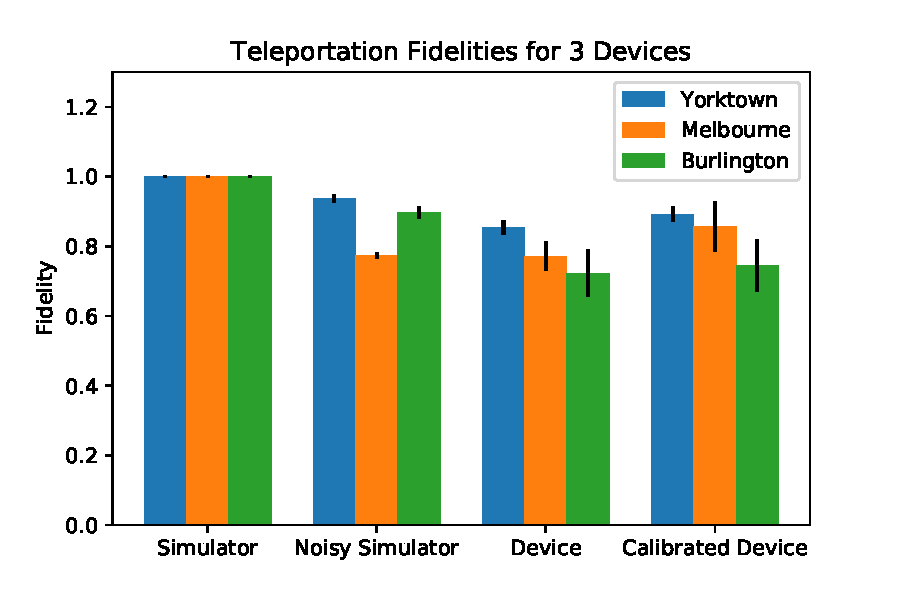
\includegraphics[width=0.48\textwidth]{images/results/teleport_histogram.pdf}
	\caption{Fidelity results for the Teleportation protocol. Error bars are
		estimated by taking the variance over 15 runs of 8,192 shots each (a total of
		122,880 shots). All simulation fidelities are within statistical error of
		unity.}
	\label{fig:teleport_histogram}
\end{figure}

The noise model captures the error in the Burlington device much less
accurately. We would expect that Burlington would perform almost as well as
Yorktown from the estimates on the noisy simulator, but in fact it performs the
worst of the three. We suspect, as will be described in more detail below, that
this is a consequence of the number of gates needed to implement the circuit on
the real device.

In order to check the readout calibration, it is useful to compare Pauli sets of
the different outcomes, which we can see in Fig. \ref{fig:tele_paulis}.

\begin{figure}[h!]
  \begin{subfigure}{.5\textwidth}
    \centering
    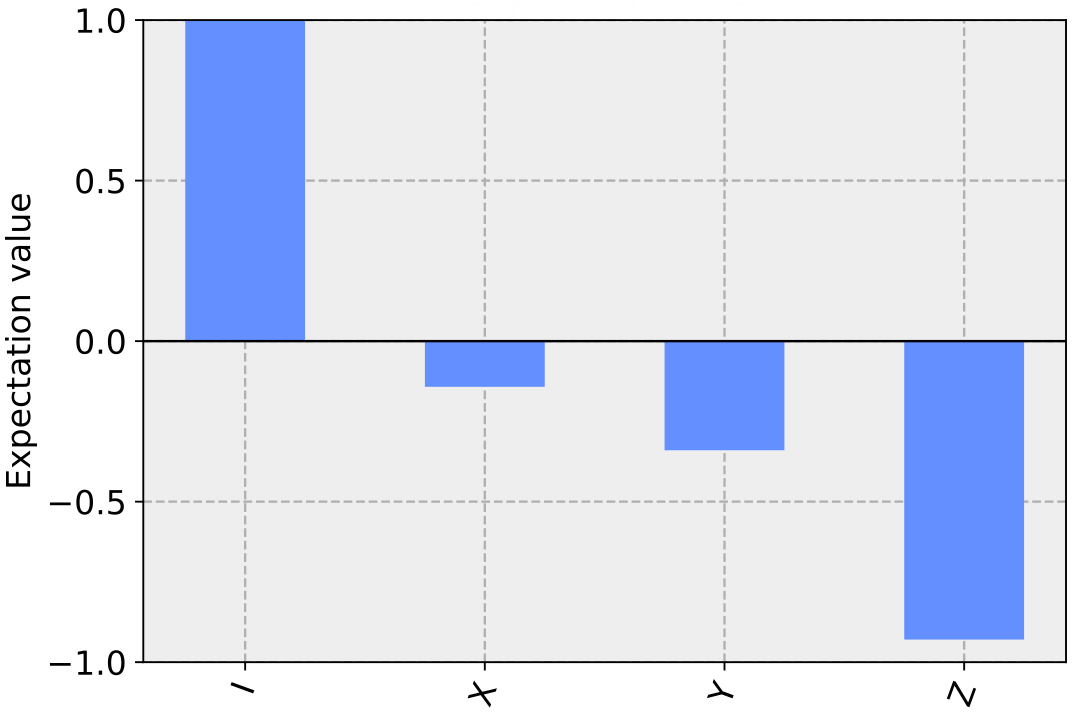
\includegraphics[width=.8\linewidth]{images/results/tele_pauli_sim.png}
    \caption{The expected Pauli set.}
    \label{fig:tele_pauli_sim}
  \end{subfigure}
  \newline
  \begin{subfigure}{.5\textwidth}
    \centering
    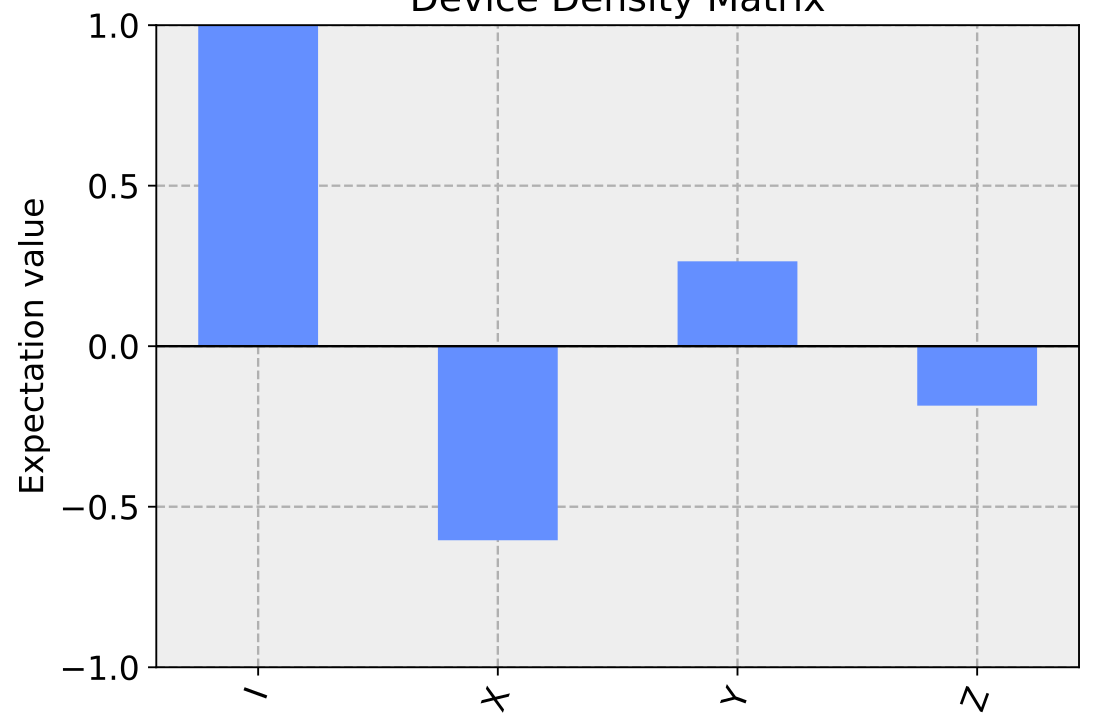
\includegraphics[width=.8\linewidth]{images/results/tele_pauli_dev.png}
    \caption{The output Pauli set for the device.}
    \label{fig:tele_pauli_dev}
  \end{subfigure}
  \newline
  \begin{subfigure}{.5\textwidth}
    \centering
    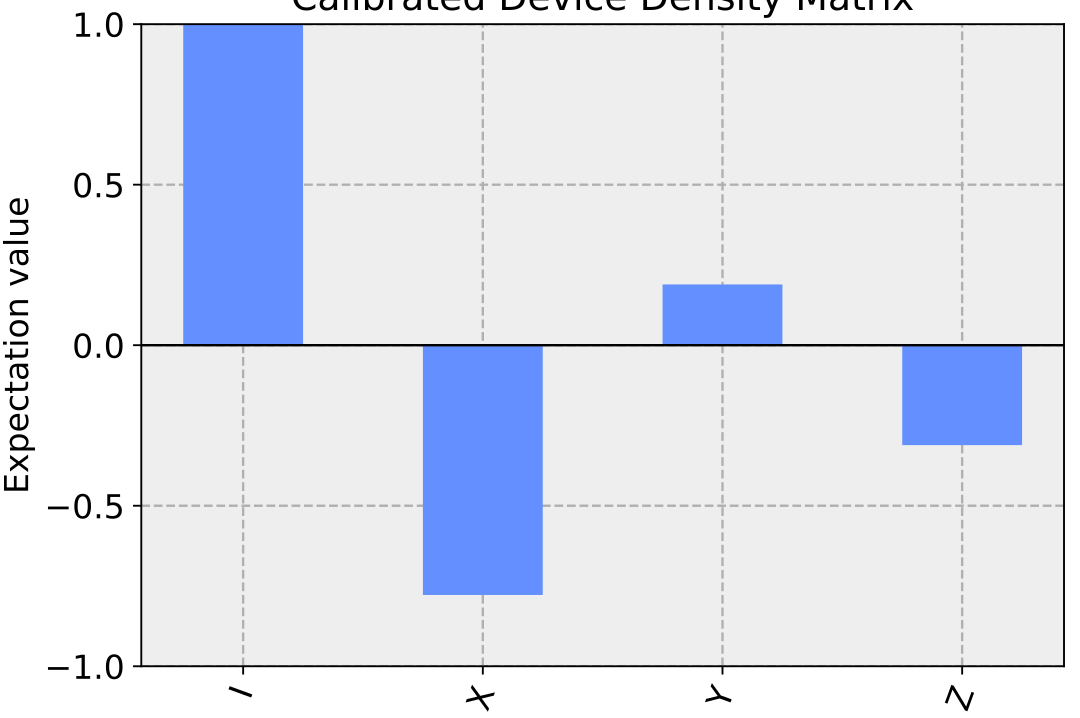
\includegraphics[width=.8\linewidth]{images/results/tele_pauli_cal.png}
    \caption{The calibrated device Pauli set.}
    \label{fig:tele_pauli_dev}
  \end{subfigure}
  \caption{The expectation values match those we expect after calibrating for
readout error. Errors in measurement contribute greatly to the low fidelity of
our final states. The type of correction seen in the figures above accounts for
the increased fidelity for the calibrated device in Fig.
\ref{fig:teleport_histogram}. Data plotted here is taken for 8192 shots on the
Melbourne backend.}
  \label{fig:tele_paulis}
\end{figure}

% This thing here is to test a full size picture don't delete.
% \begin{figure*}
%   \centering
%   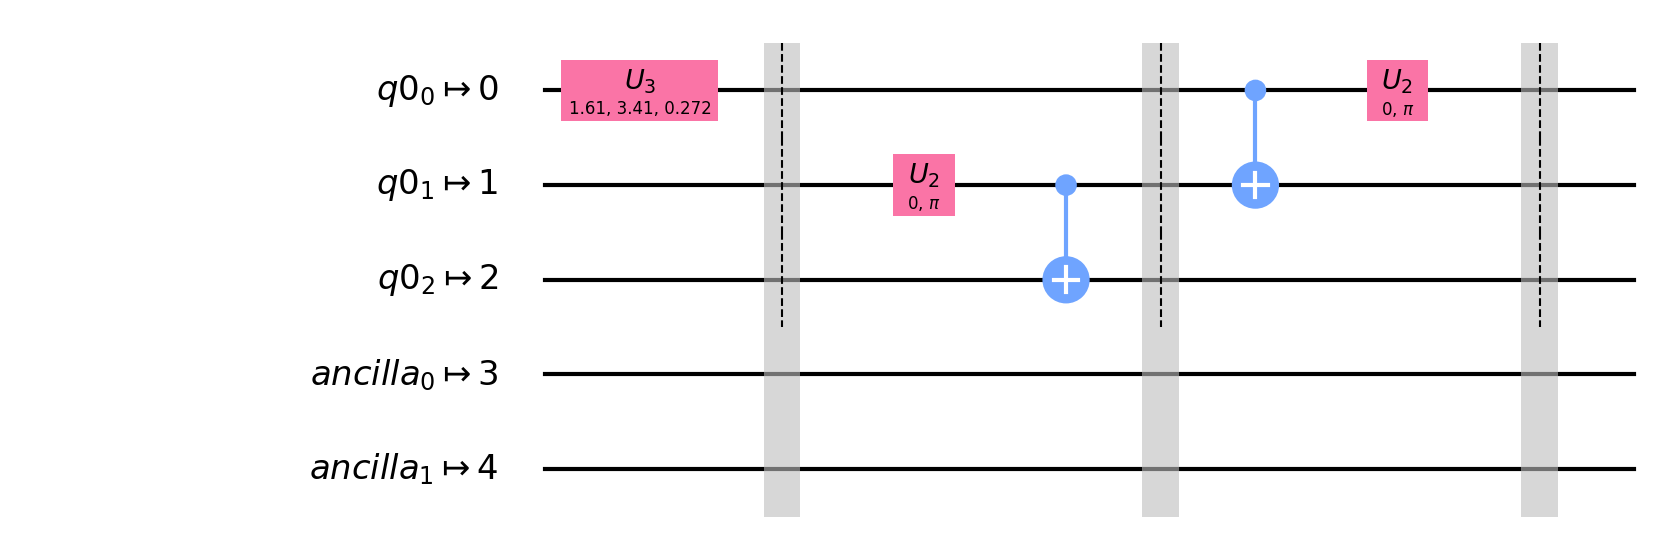
\includegraphics[width=\textwidth]{images/teleport_ibmqx2.png}
%   \caption{The most densely connected 5-qubit device at IBM Q. As we will see,
%     equally as important as the single-qubit and CNOT error rates is the degree of
%     connectivity in a device. Figure from \cite{ibmq_yorktown}.}
%   \label{fig:yorktown_connections}
% \end{figure*}

\subsection{Entanglement Swapping}
As for entanglement swapping, we first look at the main result of the
entanglement swapping circuit in Fig. \ref{fig:swap_histogram}.

\begin{figure}[h] \centering
  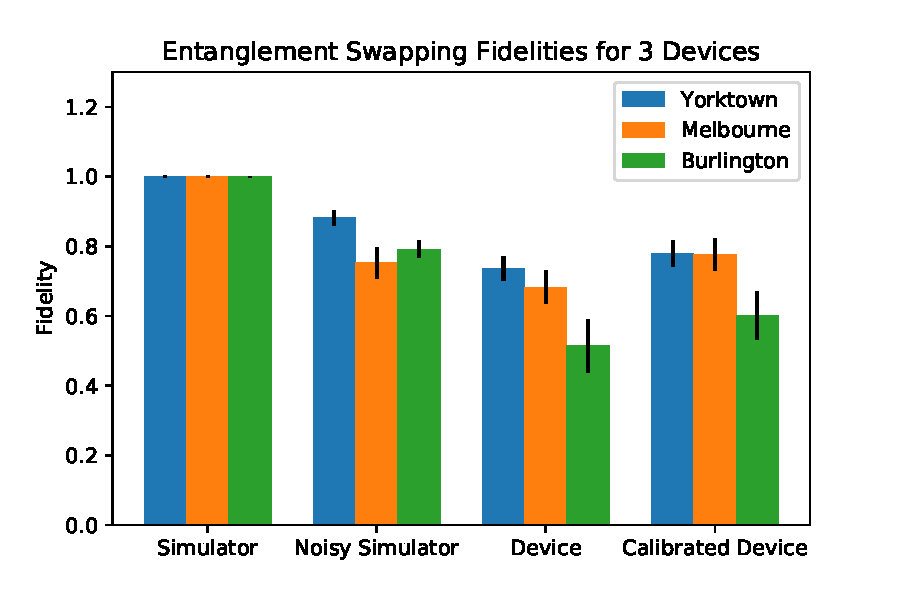
\includegraphics[width=0.48\textwidth]{images/results/swap_histogram.pdf}
	\caption{Fidelity results for the Entanglement Swapping protocol. Error bars
    are estimated by taking the variance over 15 runs of 8,192 shots each (a total
    of 122,880 shots).}
	\label{fig:swap_histogram}
\end{figure}

The fidelity measurements are done with a random generated state and a
$\ket{\Phi^+}$ Bell-state instead of the regular entanglement swapping circuit
where we only swap Bell-states. Again we see that the simulation fidelities are
1 within statistical error, which means that the swapping of initial Bell-states
are done correctly using tomography to construct the final state, and
post-measurement selection to transform specified results to specific basis. As
we expected fidelities from the noisy simulator are much better than results
from all the devices. The main difference between teleportation is the fact that
Burlington's performance is worse while the other devices give similar (or
slightly worse) fidelities. We could predict this behavior since the circuit
uses more qubits and hence the total error (due to operations and the qubits
themselves) will be more significant. Also note that using the two-qubit state
tomography method (see section \ref{two-qubit} of \nameref{theory}) results in
an overall improvement of the fidelity. From this calculation we can conclude
that a significant part of the error is due to readout error. In order to have a
more detailed insight into the readout error correction we look at the Pauli
sets in Fig. \ref{fig:swap_paulis} to analyze the error calibration in different
basis. For this result we looked the swapping process of two $\ket{\Phi^+}$
Bell-states. We conclude that the error correction is too insignificant to
derive at the expected Pauli set results (even though there is a small
improvement).

\begin{figure}[h!]
	\begin{subfigure}{.5\textwidth} \centering % include first image
		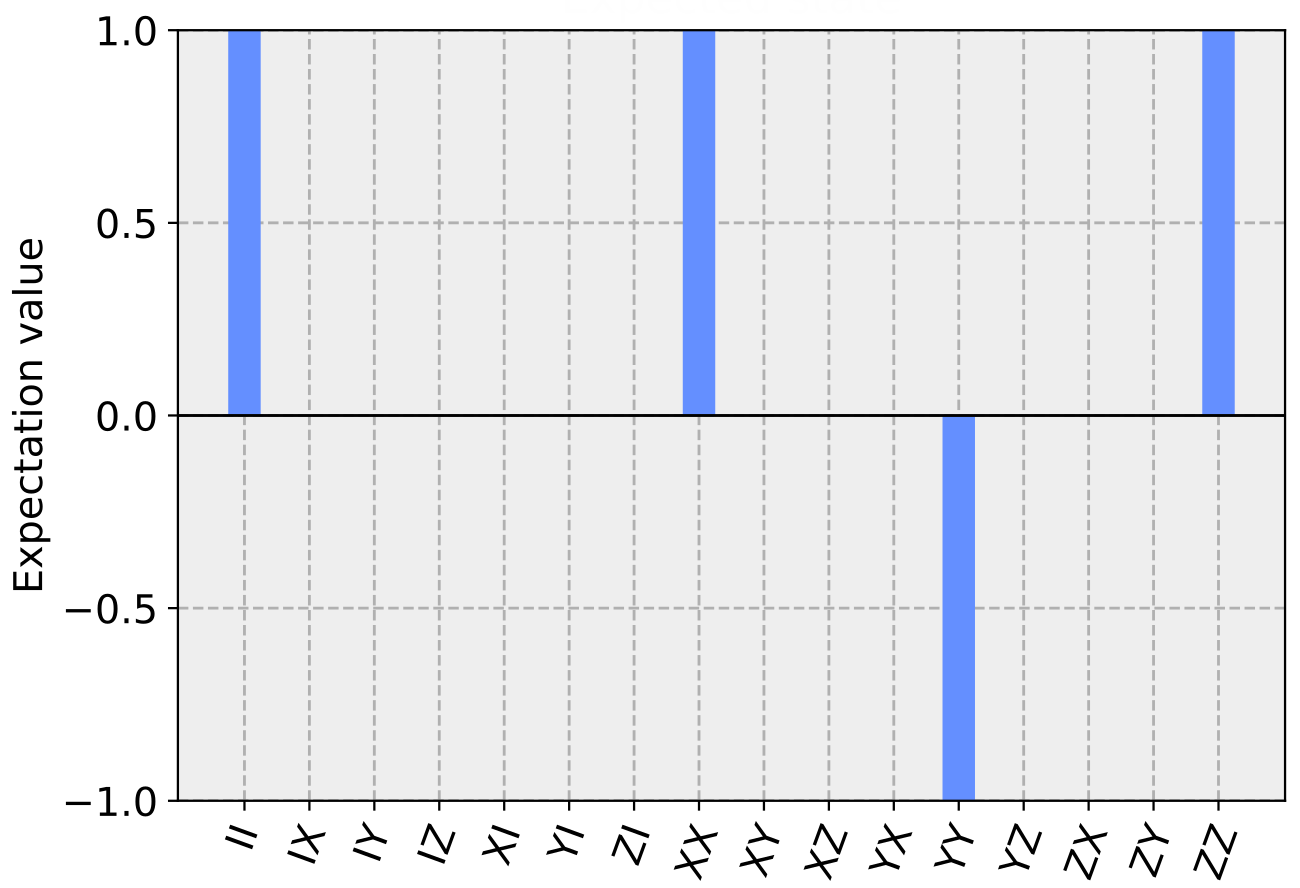
\includegraphics[width=.8\linewidth]{images/results/swap_pauli_sim.png}
		\caption{The expected Pauli set.}
		\label{fig:swap_pauli_sim}
	\end{subfigure} \newline
	\begin{subfigure}{.5\textwidth} \centering % include second image
		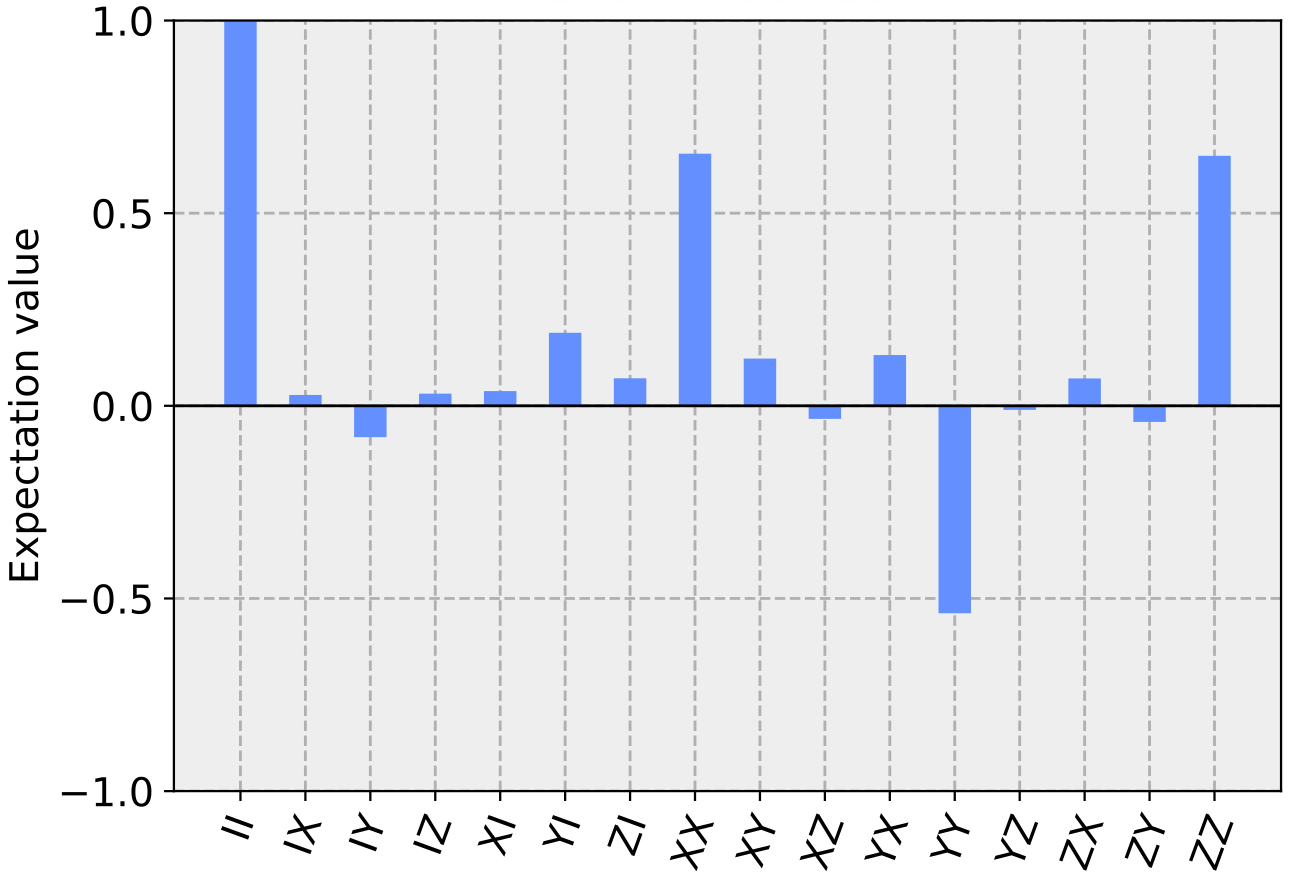
\includegraphics[width=.8\linewidth]{images/results/swap_pauli_dev.png}
		\caption{The output Pauli set for the device.}
		\label{fig:swap_pauli_dev}
	\end{subfigure} \newline
	\begin{subfigure}{.5\textwidth} \centering % include second image
		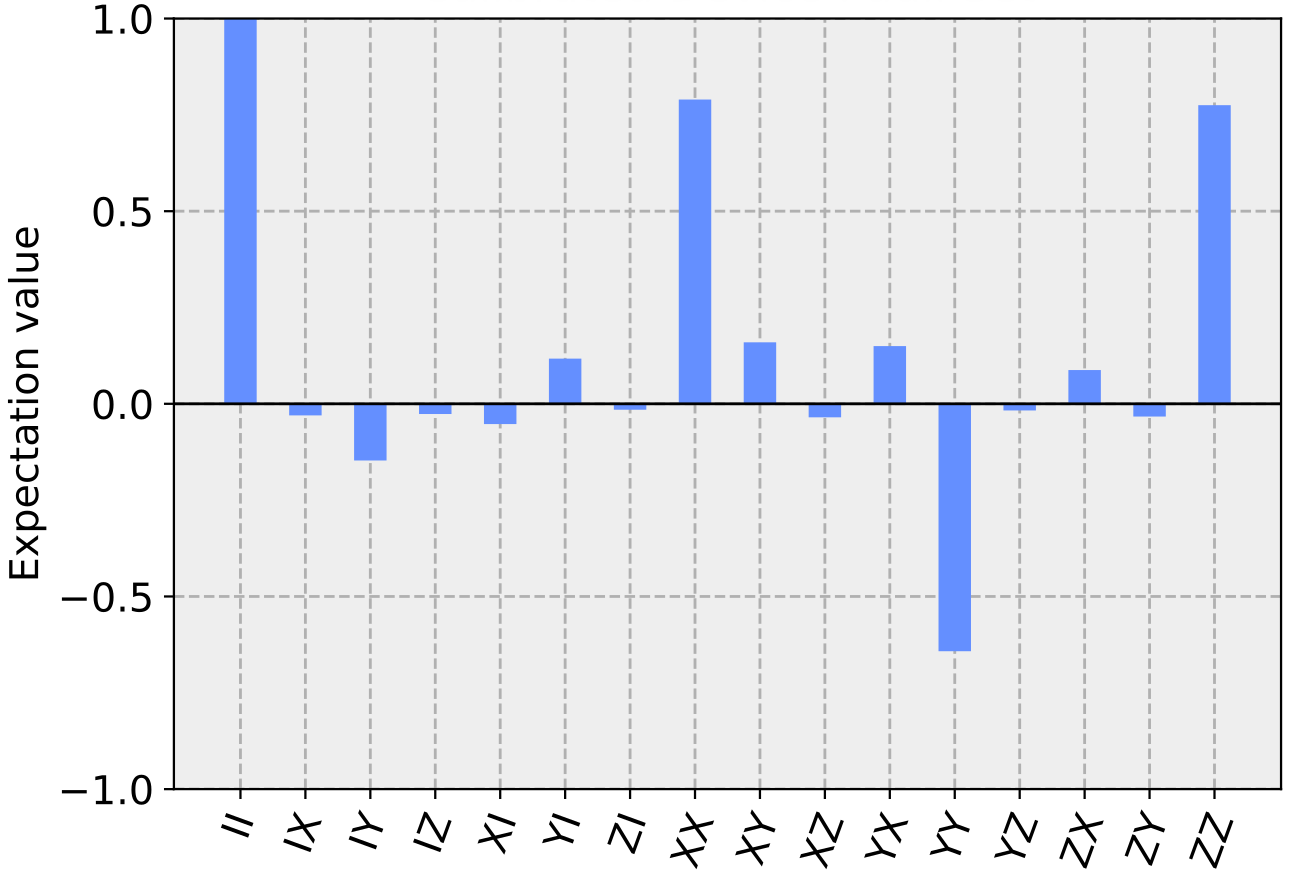
\includegraphics[width=.8\linewidth]{images/results/swap_pauli_cal.png}
		\caption{The calibrated device Pauli set.}
		\label{fig:swap_pauli_dev}
	\end{subfigure}
	\caption{ Pauli set entanglement swapping results for the ideal simulator, the
device and the calibrated device. The type of correction seen in the figures
above accounts for the increased fidelity for the calibrated device in Fig.
\ref{fig:swap_histogram}. Data plotted here is taken for 8192 shots on the
Melbourne backend.}
	\label{fig:swap_paulis}
\end{figure}

Next we take a more in depth look into the different states by
analyzing the density matrix plots, which are presented in Fig.
\ref{fig:swap_density}. From these density plots we conclude that the device
calibration improves the final state so that it closer represents the
$\ket{\Phi^+}$ state.

\begin{figure}
	\begin{subfigure}{.5\textwidth} \centering % include first image
		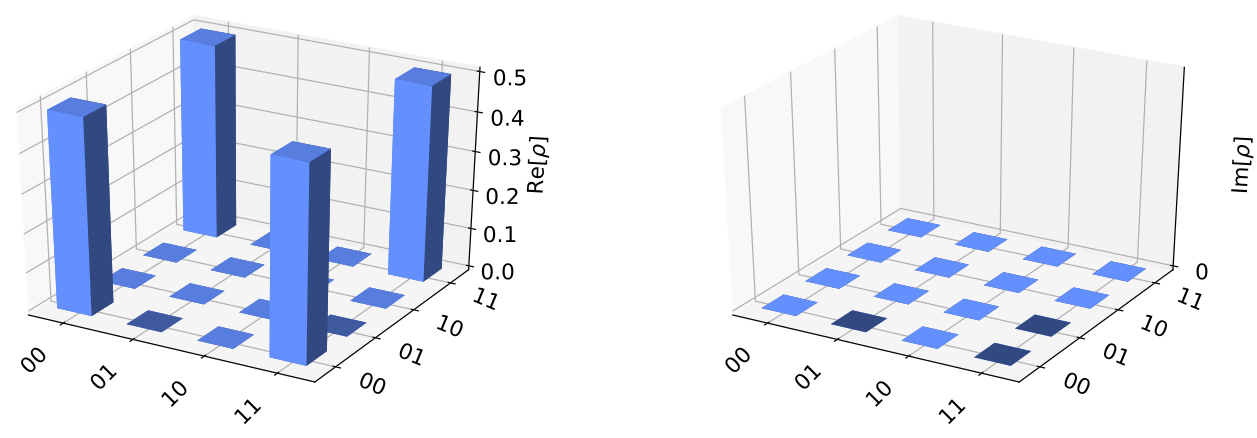
\includegraphics[width=.8\linewidth]{images/results/swap_density_sim.png}
		\caption{The expected Density matrix.}
		\label{fig:swap_density_sim}
	\end{subfigure} \newline
	\begin{subfigure}{.5\textwidth} \centering % include second image
		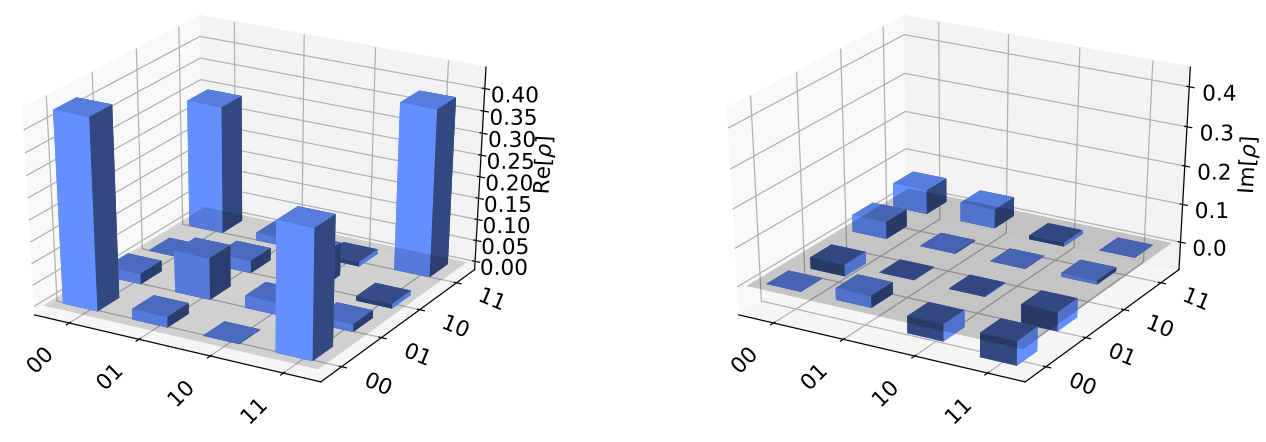
\includegraphics[width=.8\linewidth]{images/results/swap_density_dev.png}
		\caption{The output Density matrix for the device.}
		\label{fig:swap_density_dev}
	\end{subfigure} \newline
	\begin{subfigure}{.5\textwidth} \centering % include second image
		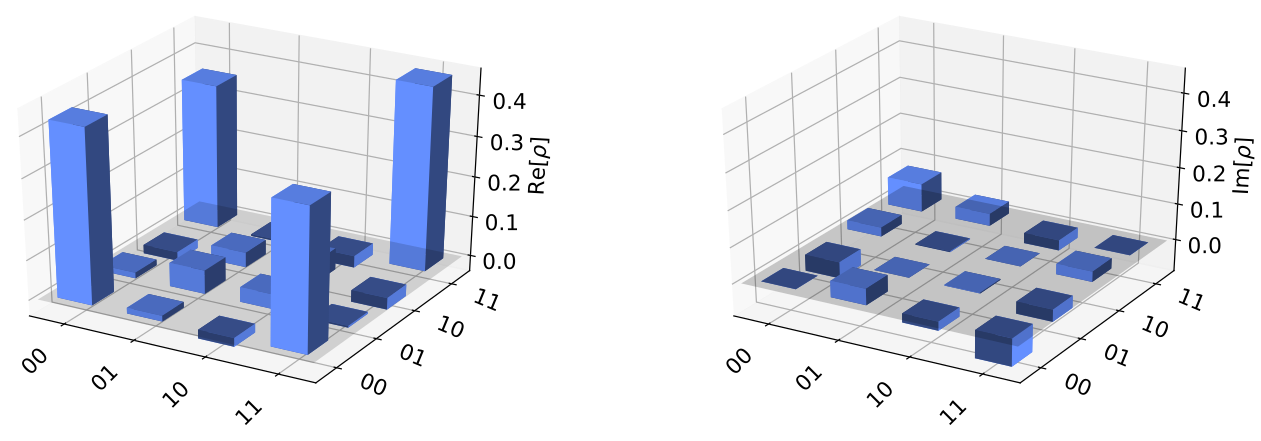
\includegraphics[width=.8\linewidth]{images/results/swap_density_cal.png}
		\caption{The calibrated device Density matrix.}
		\label{fig:swap_density_dev}
	\end{subfigure}
	\caption{ The entanglement swapping density matrices for the ideal simulator,
the device and the calibrated device. Data plotted here is taken for 8192 shots
on the Melbourne backend. }
	\label{fig:swap_density}
\end{figure}

\subsection{Entanglement Purification}
\subsection{Grover's Algorithm}


%%% Local Variables:
%%% mode: latex
%%% TeX-master: "report"
%%% End: